\documentclass{beamer}

\graphicspath{{images/}}

\usepackage{appendixnumberbeamer}

\usepackage{datetime}
\newdate{defensedate}{6}{11}{2017}

\usepackage{minted}

\usetheme[sectionpage=progressbar,subsectionpage=progressbar,numbering=fraction,
          progressbar=foot]{metropolis}

\usepackage{amssymb}

% \usepackage[inline]{enumitem}

\title{Scheduling of Synchronous Data Flow Models onto Scratchpad Memory-Based Embedded Processors}

\date{\displaydate{defensedate}}
\author{%
  Simon Bihel\hfill\url{simon.bihel@ens-rennes.fr} \\
}
\institute{%
  University of Rennes I \\
  \'Ecole Normale Sup\'erieure de Rennes
}

\begin{document}

\maketitle

\begin{frame}{Table of contents}
  \setbeamertemplate{section in toc}[sections numbered]
  \tableofcontents[hideallsubsections]
\end{frame}


\section{Problem Statement}

\begin{frame}{Scratchpad Memory (SPM)}
  Replacing caches by a bit of memory explictly managed by the user.
\end{frame}

\begin{frame}{Stream Applications}
  \begin{columns}
    \begin{column}{0.4\textwidth}
      \begin{center}
        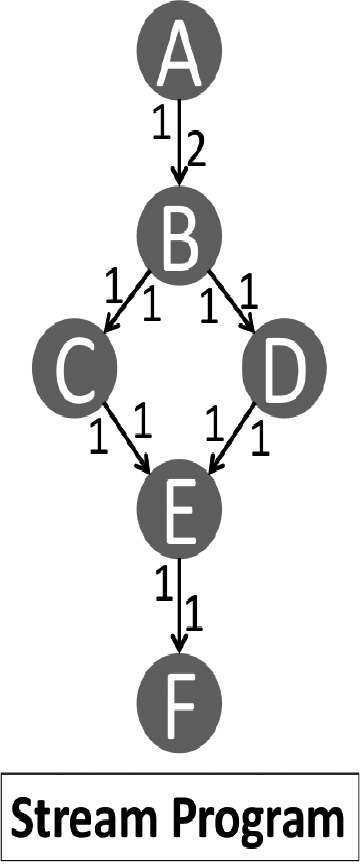
\includegraphics[height=0.85\textheight]{fig2_1}
      \end{center}
    \end{column}
    \begin{column}{0.6\textwidth}
      \begin{itemize}
        \item Synchronous Data Flow graph of \alert{actors}
        \item Actors process and produce \alert{tokens}
      \end{itemize}
    \end{column}
  \end{columns}
\end{frame}

\begin{frame}{Output Schedule}
  \begin{columns}
    \begin{column}{0.4\textwidth}
      \begin{center}
        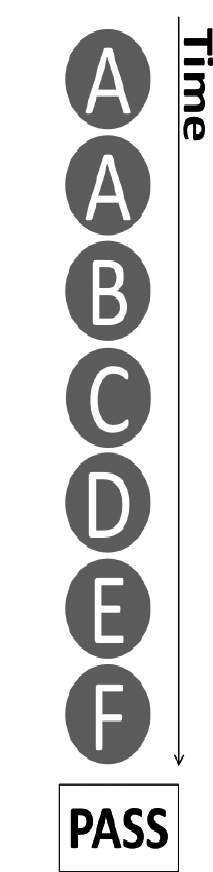
\includegraphics[height=0.85\textheight]{fig1_2}
      \end{center}
    \end{column}
    \begin{column}{0.6\textwidth}
      \begin{itemize}
        \item Sequential execution
        \item Periodical
      \end{itemize}
    \end{column}
  \end{columns}
\end{frame}

\begin{frame}{SPM partition}
  \begin{columns}
    \begin{column}{0.55\textwidth}
      \begin{center}
        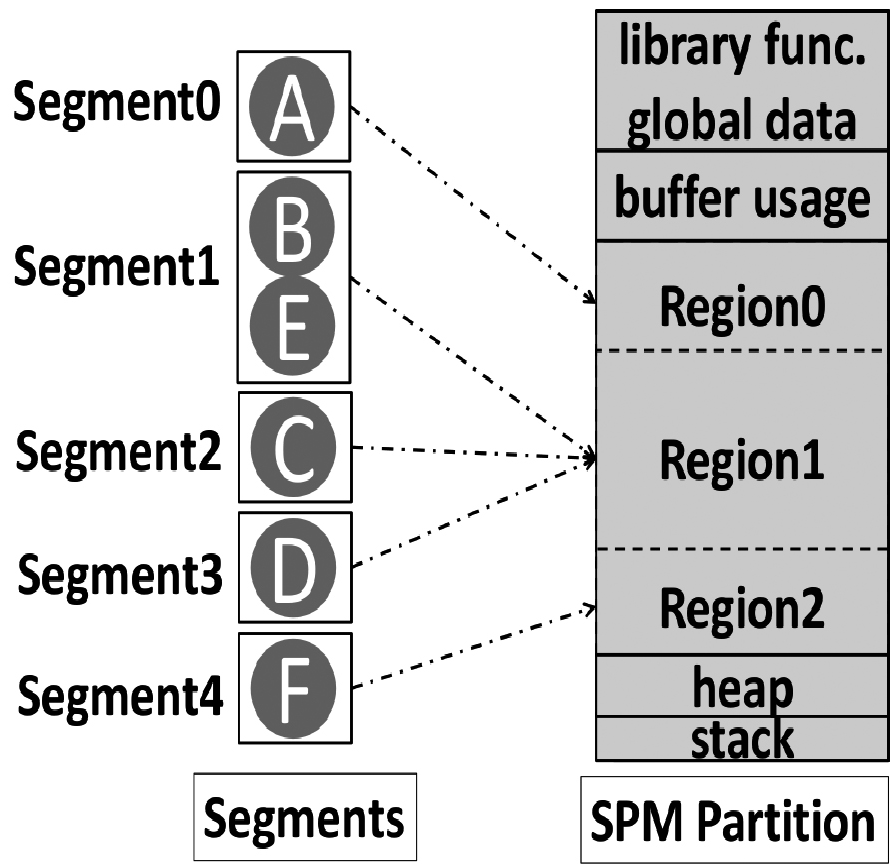
\includegraphics[height=0.75\textheight]{fig2_2}
      \end{center}
    \end{column}
    \begin{column}{0.45\textwidth}
      \begin{description}
        \item[Buffer Usage] Storing data
        \item[Regions] One segment present at a time
        \item[Segments] All actors present at the same time
      \end{description}
    \end{column}
  \end{columns}
\end{frame}

\begin{frame}{Code Overlay}
  Not all actors code can reside in the SPM\@:
  \begin{itemize}
    \item store extraneous actors in main memory;
    \item load actor before execution.
  \end{itemize}

  \begin{description}
    \item[Code Overlay] replacing a segment by another.
  \end{description}

  Processor is idle during memory access to fetch code.
\end{frame}

\begin{frame}{Example}
  \begin{columns}
    \begin{column}{0.35\textwidth}
      \begin{center}
        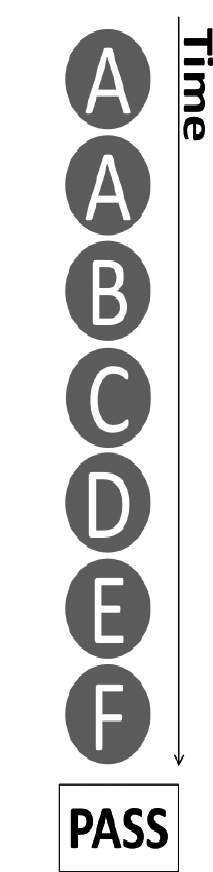
\includegraphics[height=0.75\textheight]{fig1_2}
      \end{center}
    \end{column}
    \begin{column}{0.7\textwidth}
      \begin{center}
        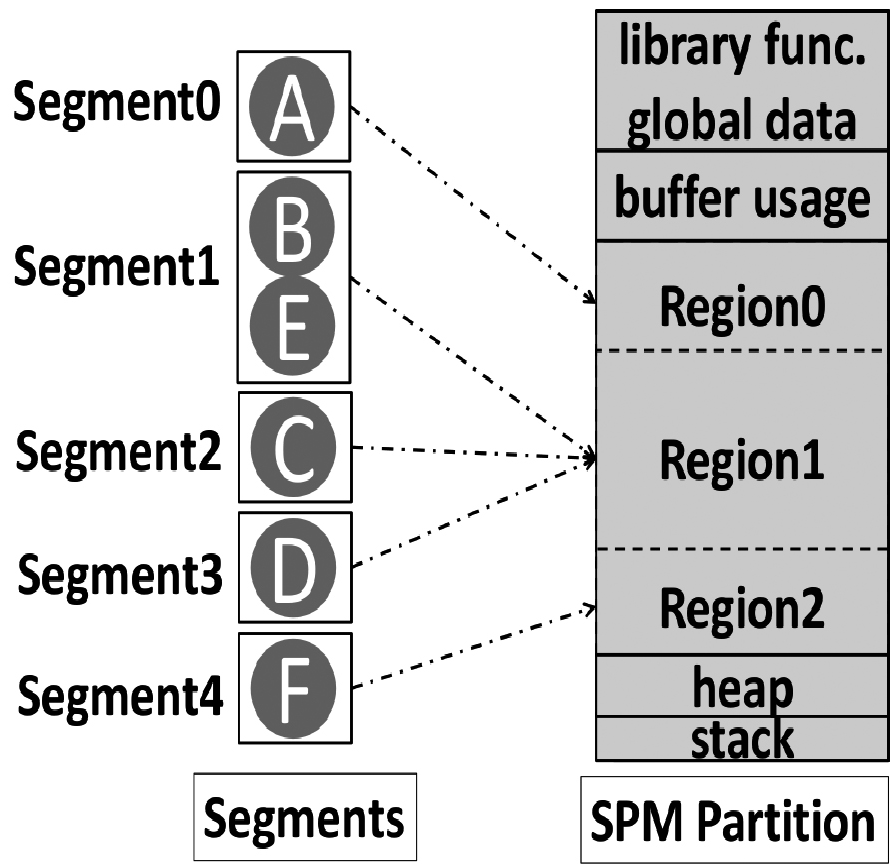
\includegraphics[height=0.75\textheight]{fig2_2}
      \end{center}
    \end{column}
  \end{columns}
\end{frame}

\begin{frame}{Objectives}
  Problem: decide on the best PASS, regions and segments for the least idle time.

  Two proposed properties to focus on:
  \begin{description}
    \item[Buffer Usage] reducing maximum of simultaneous tokens to free space for code;
    \item[Actor Switches] grouping same actor in consecutive calls.
  \end{description}
\end{frame}


\section{Basic Heuristic}

\begin{frame}{Region Assignment}
  \begin{center}
    \hspace*{-0.1\textwidth}
    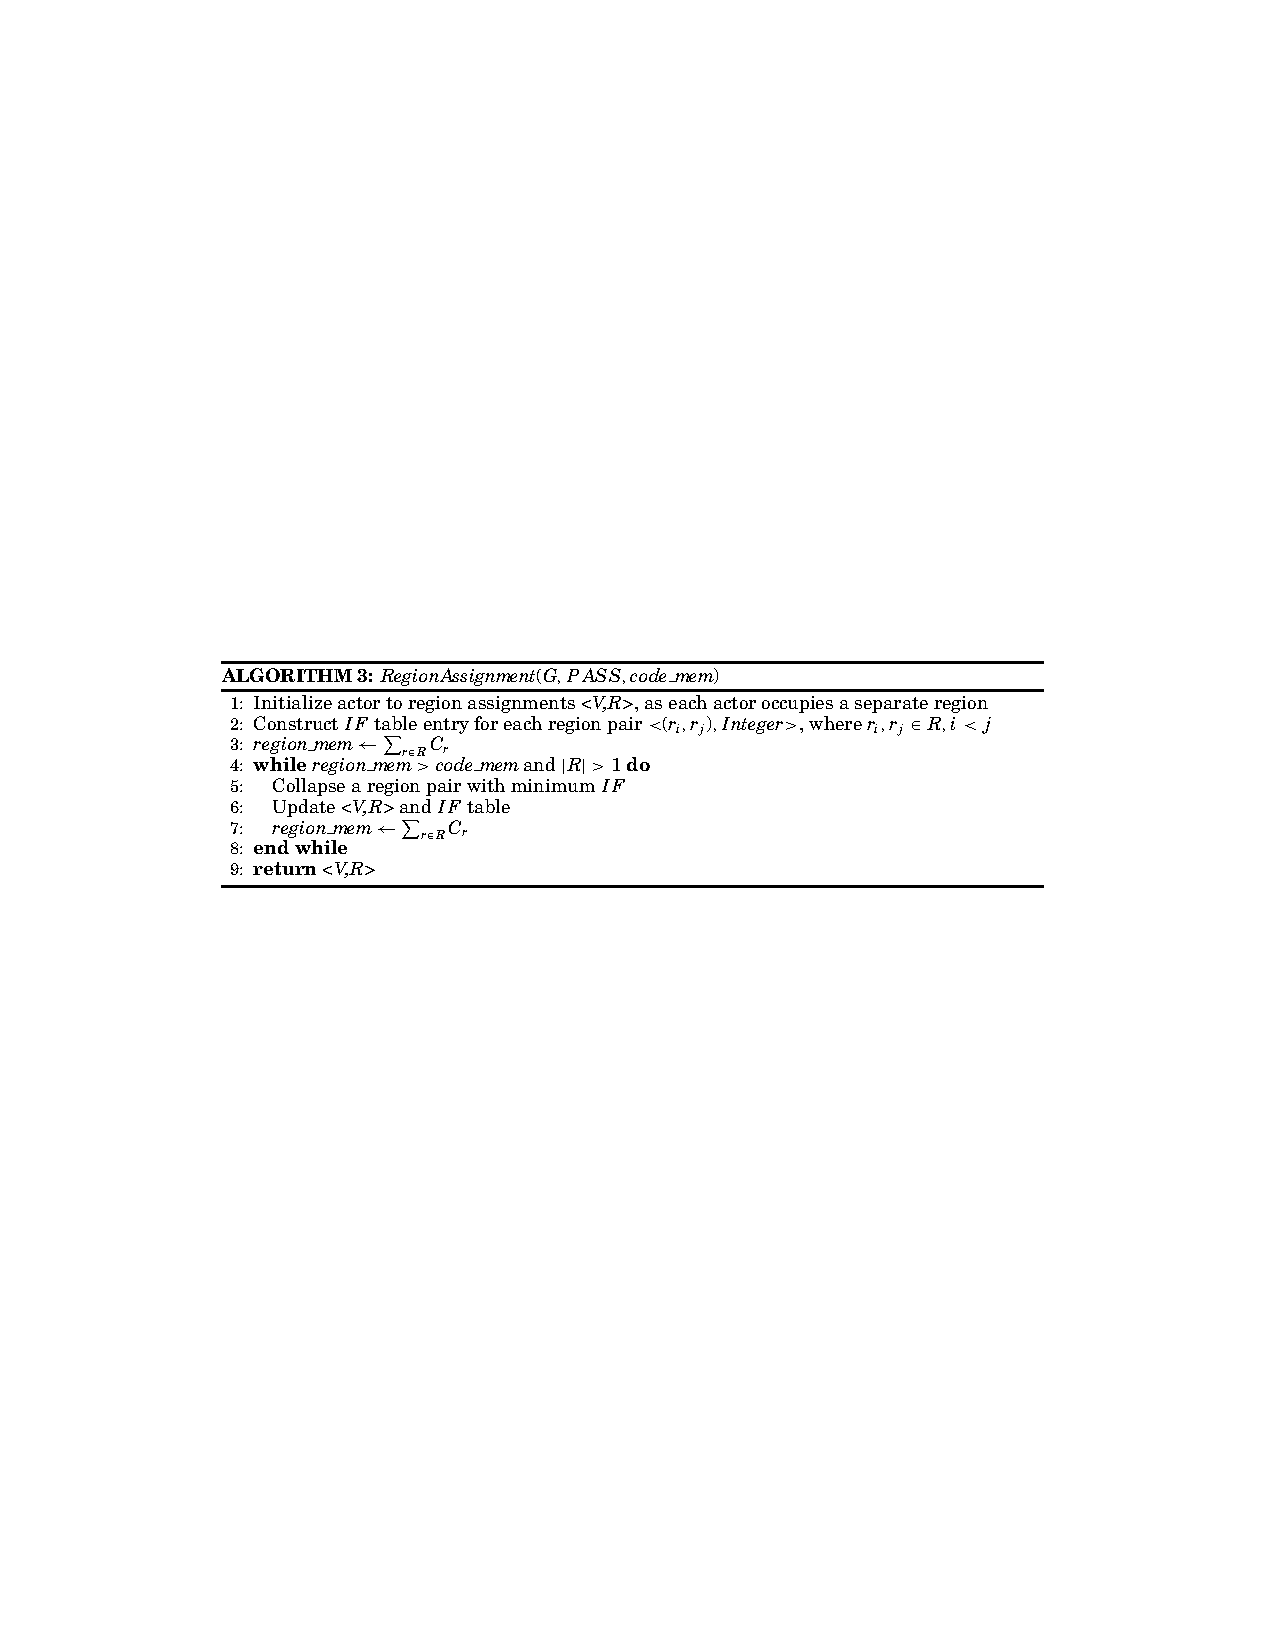
\includegraphics[width=1.2\textwidth]{algo3}
  \end{center}
  \begin{itemize}
    \item Greedy algorithm;
    \item \textit{IF} is the Interaction Factor (number of switches) between two actors.
  \end{itemize}
\end{frame}

\begin{frame}{Segmentation}
  % \begin{center}
  %   \hspace*{-0.1\textwidth}
  %   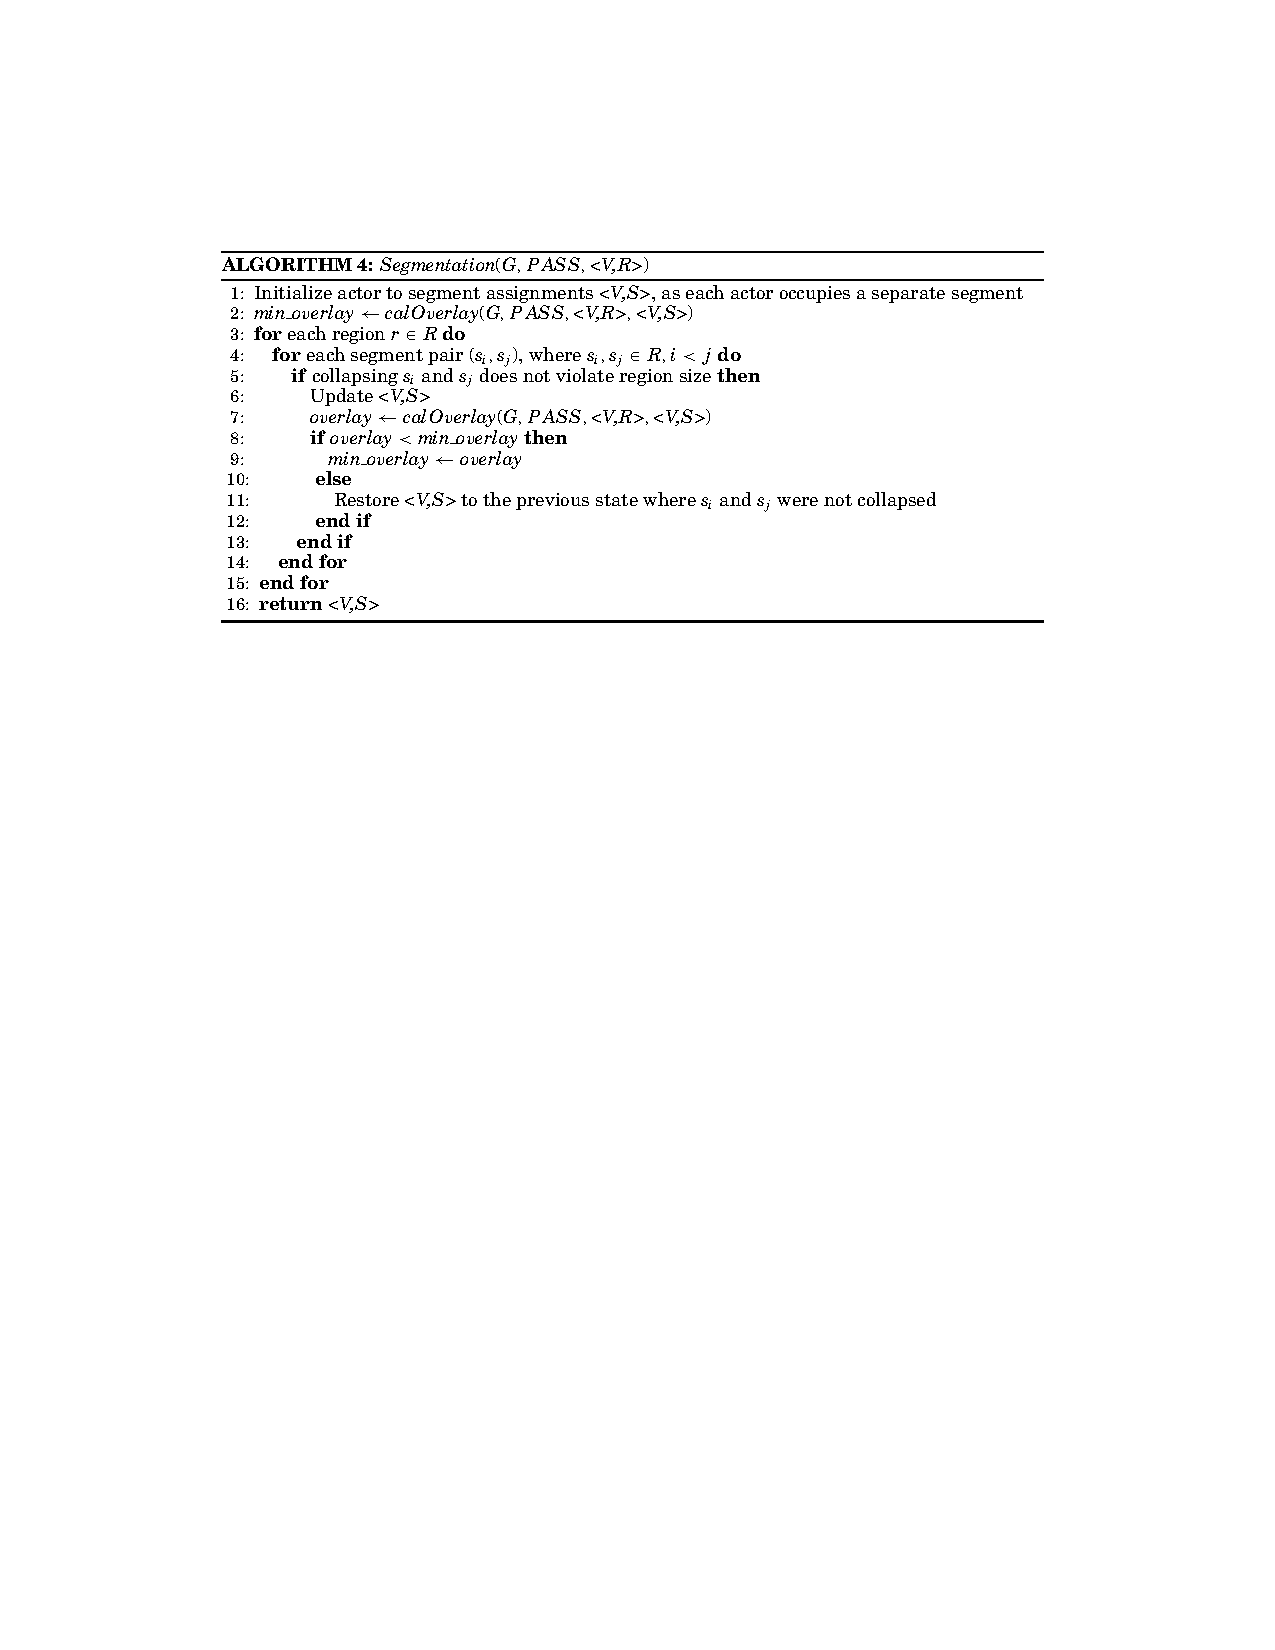
\includegraphics[width=1.2\textwidth]{algo4}
  % \end{center}
  \begin{itemize}
    \item Greedy algorithm;
    \item start with each actor with its own segment;
    \item fusion segments as long as: (i) not bigger than region size; (ii) and reduces code overlay.
  \end{itemize}
\end{frame}

\begin{frame}{Main Algorithm}
  Evolve from Minimum Buffer Schedule toward Minimum Actor Switches. % TODO why
  \begin{center}
    \hspace*{-0.1\textwidth}
    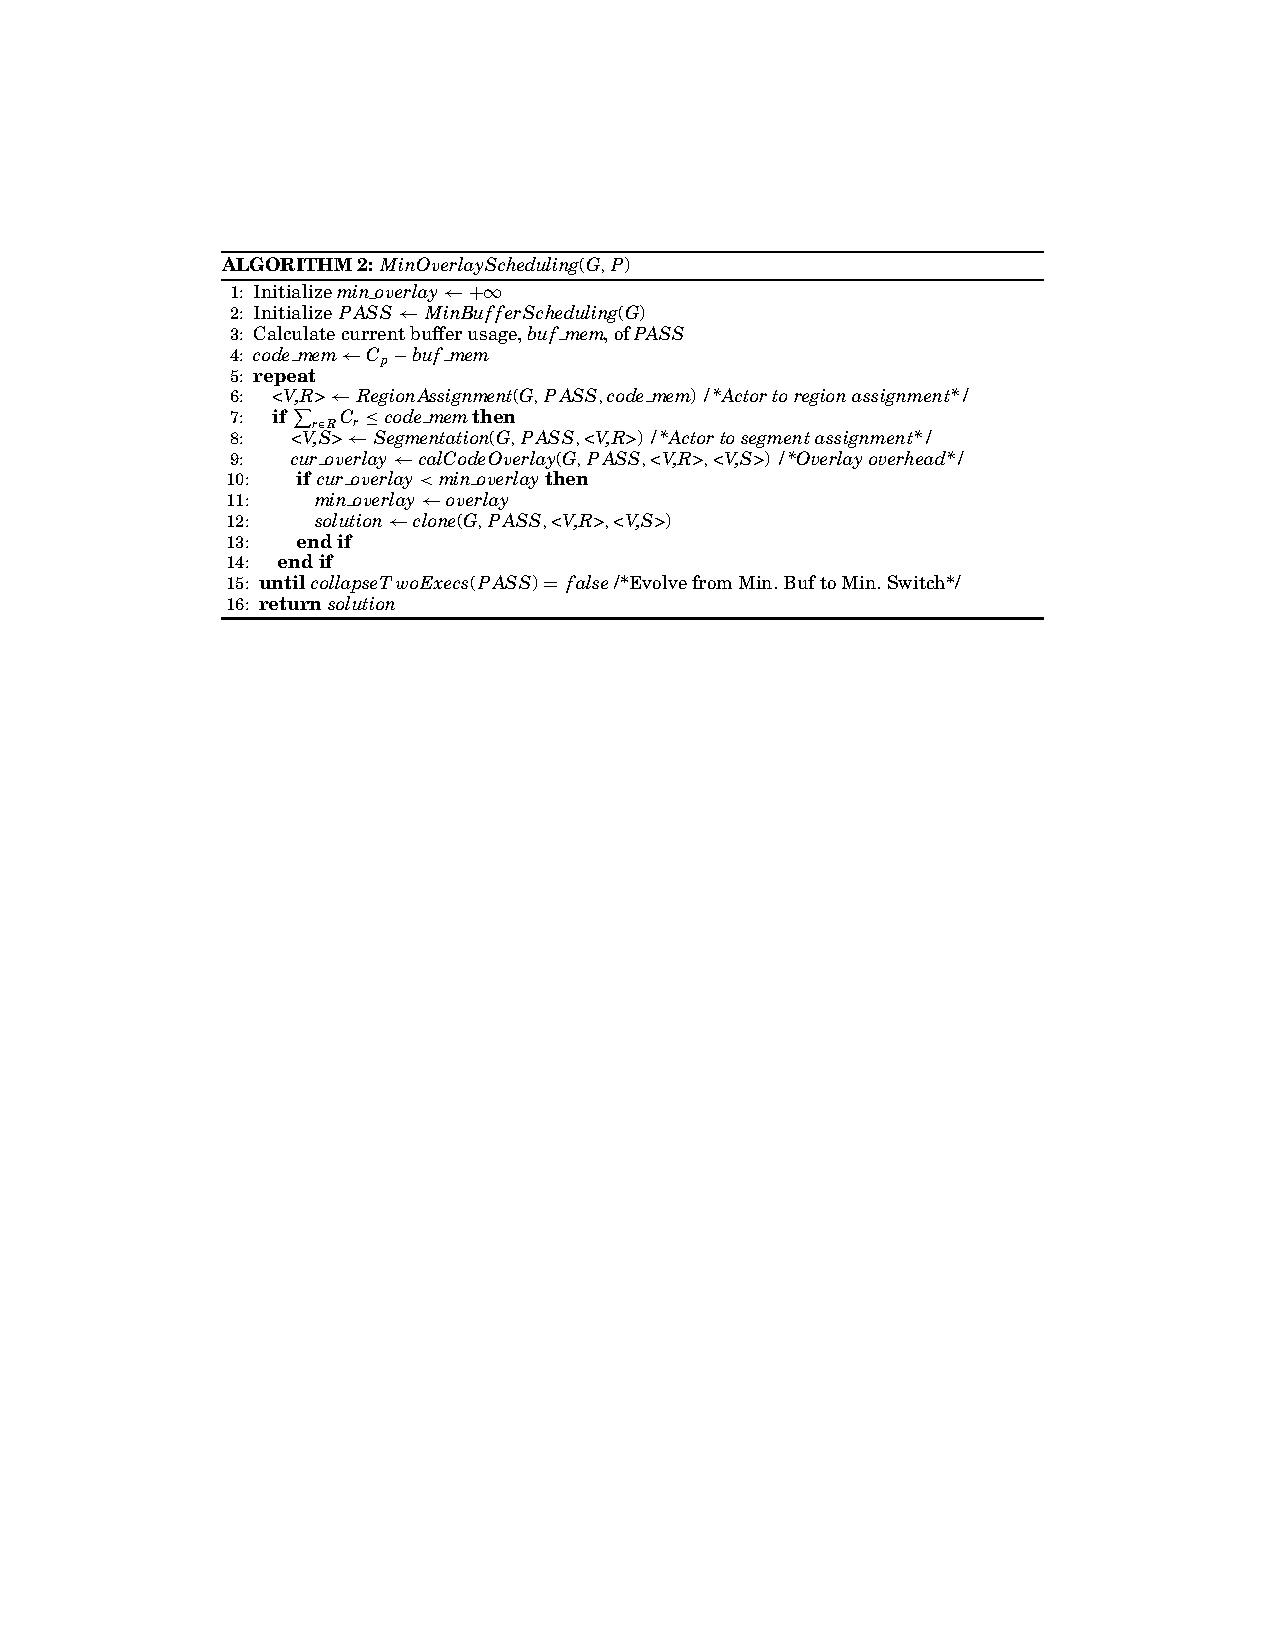
\includegraphics[width=1.2\textwidth]{algo2}
  \end{center}
\end{frame}


\section{Optimizations}

\begin{frame}{Code prefetching}
  Fetch code from main memory in advance, during the execution of an actor from another region.
\end{frame}

\begin{frame}{Data Overlay}
  Instead of keeping all tokens in the SPM, put some in the main memory until it is useful.
  \begin{itemize}
    \item Frees space for code.
  \end{itemize}
  % TODO re-read the data overlay part
\end{frame}


\section{Evaluation}

\begin{frame}{State-of-the-art comparison}
  Comparison 3-stage Integer Linear Program (Minimum Buffer Scheduling).
  \begin{center}
    \hspace*{-0.05\textwidth}
    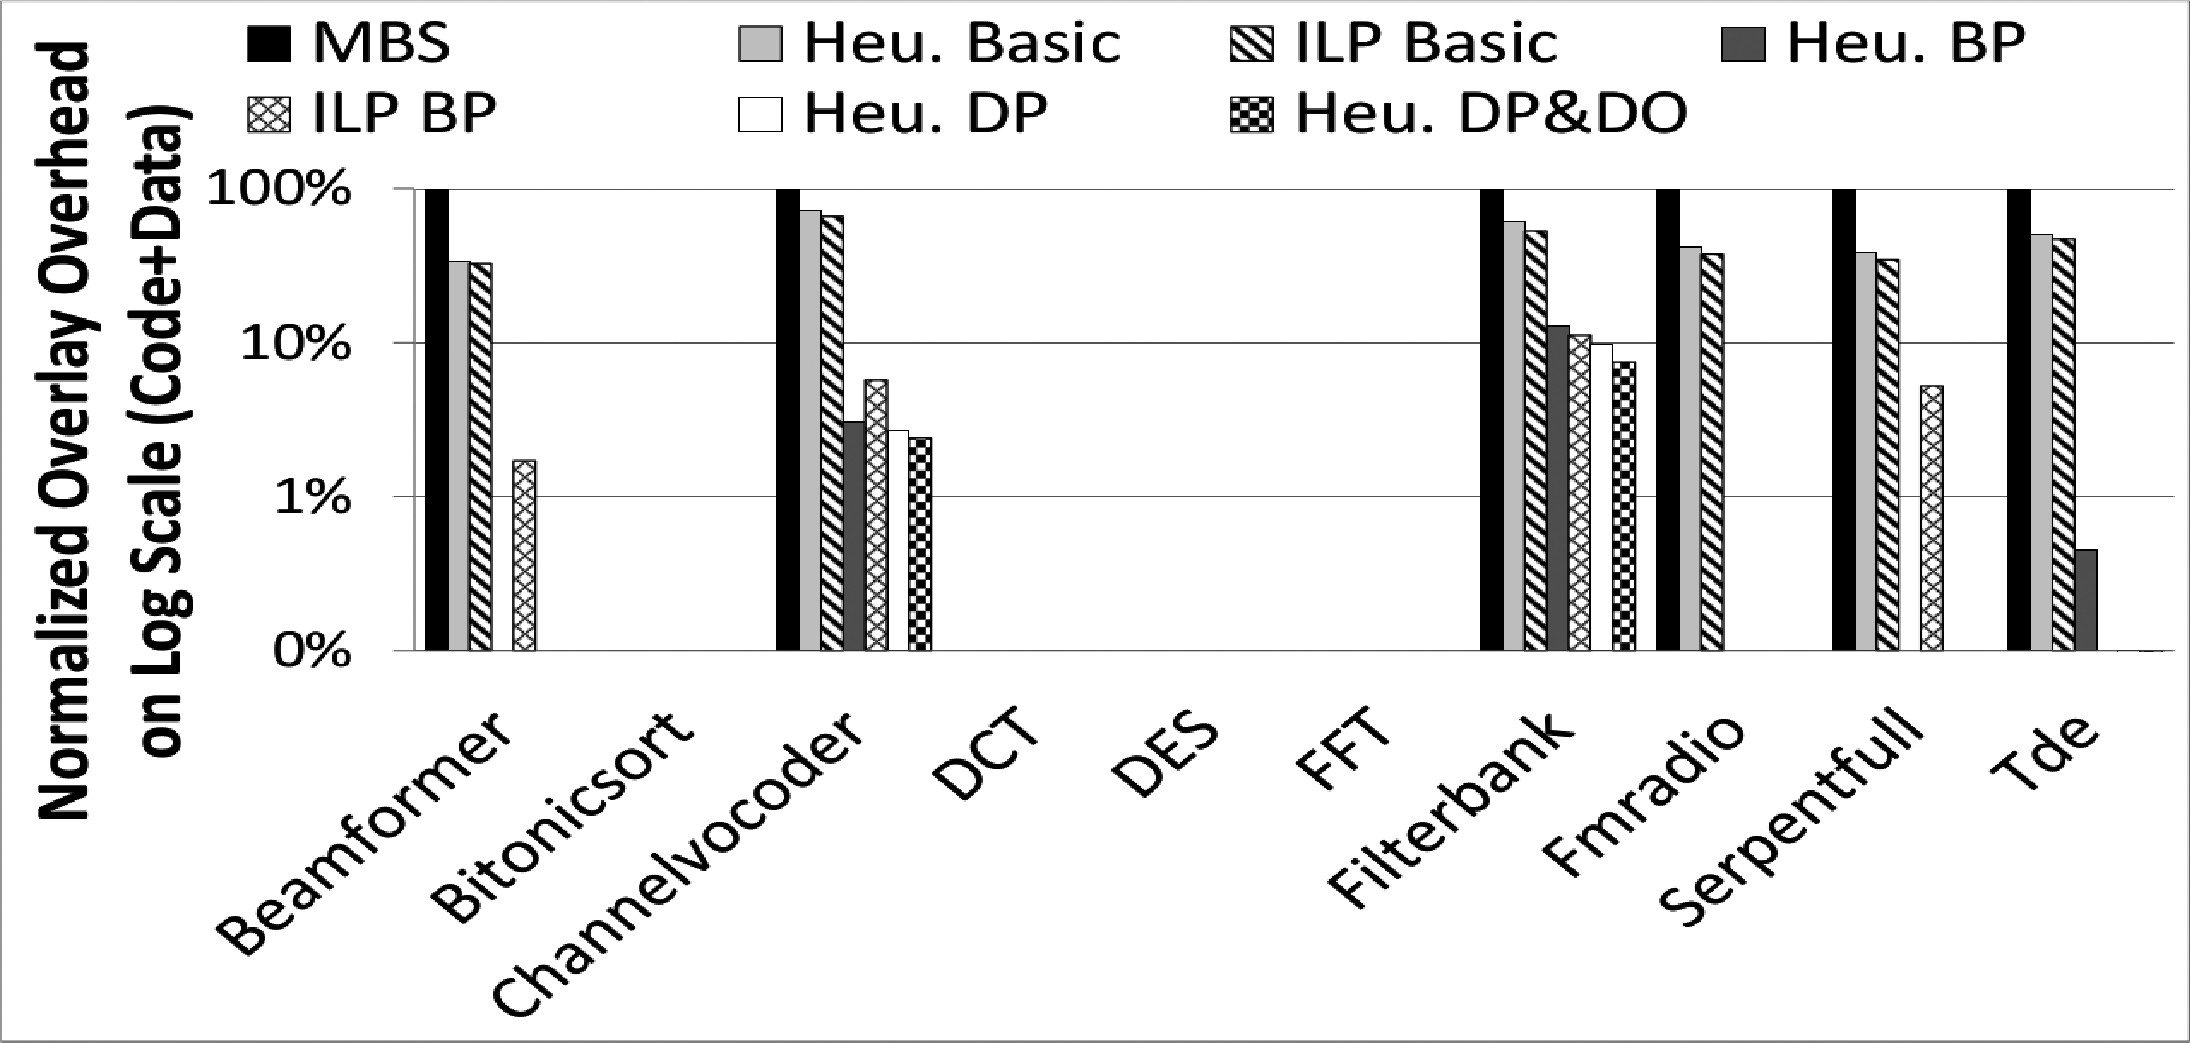
\includegraphics[width=1.1\textwidth]{fig10}
  \end{center}
\end{frame}

\begin{frame}{Optimizations impact}
  \begin{center}
    \hspace*{-0.05\textwidth}
    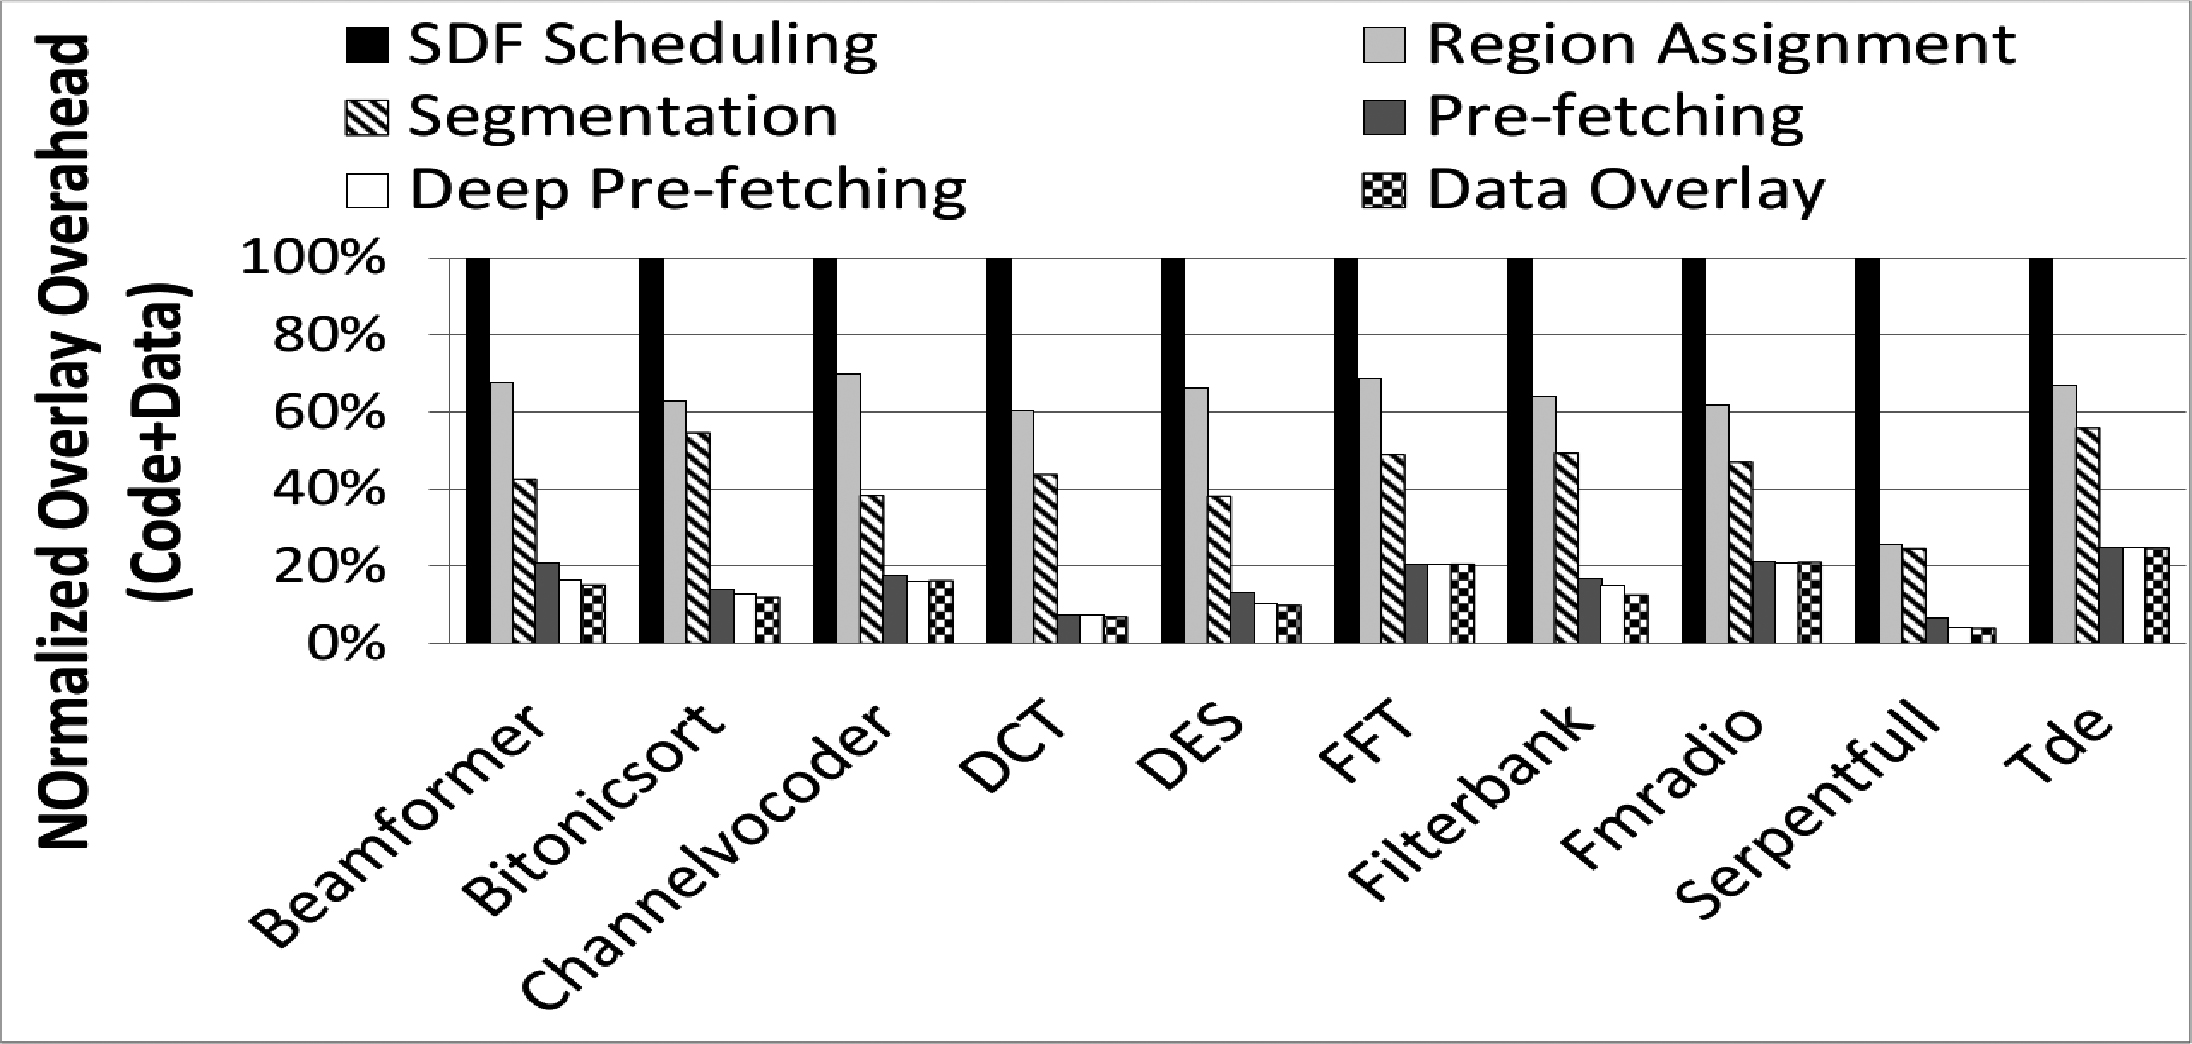
\includegraphics[width=1.1\textwidth]{fig11}
  \end{center}
\end{frame}

\begin{frame}{Heuristic Focus}
  Verify reduction of idle time by aiming for Minimum Actor Switches schedule.
  \begin{center}
    \hspace*{-0.05\textwidth}
    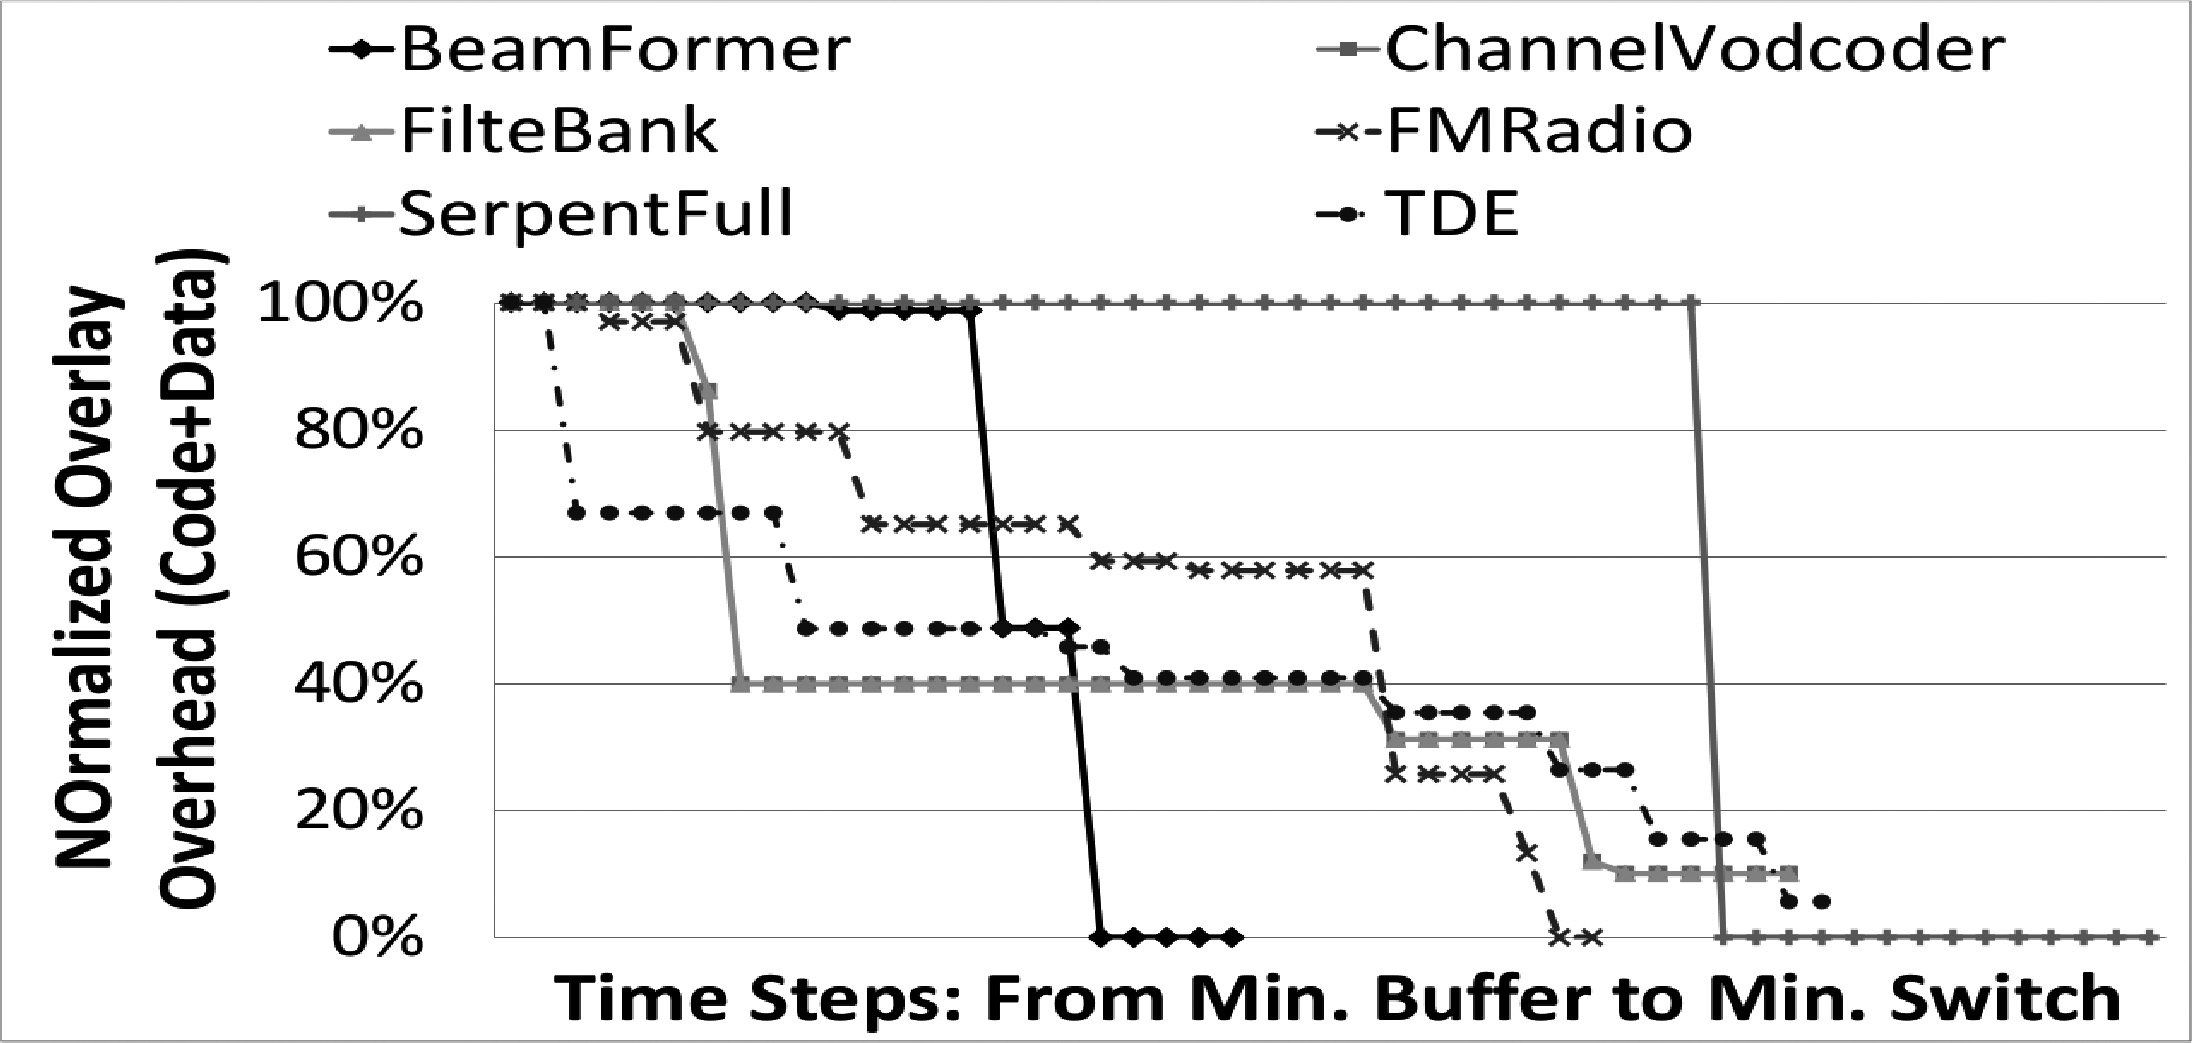
\includegraphics[width=1.1\textwidth]{fig15}
  \end{center}
\end{frame}

\begin{frame}{Architecture Scaling}
  \begin{itemize}
    \item Increasing the SPM \textit{generally} results in better results.
    \item Increasing the DMA transfer cost (simulating multi-core) renders optimizations useless.
    \item Increasing code size makes optimizations more effective (until the SPM is too small and can't run the program).
  \end{itemize}
\end{frame}


\section*{Conclusion}

\begin{frame}{Conclusion}
  \begin{itemize}
    \item Thoughtful evaluation;
    \item complexity in $O(n^5)$, no comparison of runtime with the state-of-the-art.
  \end{itemize}
\end{frame}

\appendix

\begin{frame}{Code Overlay Calculation}
  \begin{center}
    \hspace*{-0.1\textwidth}
    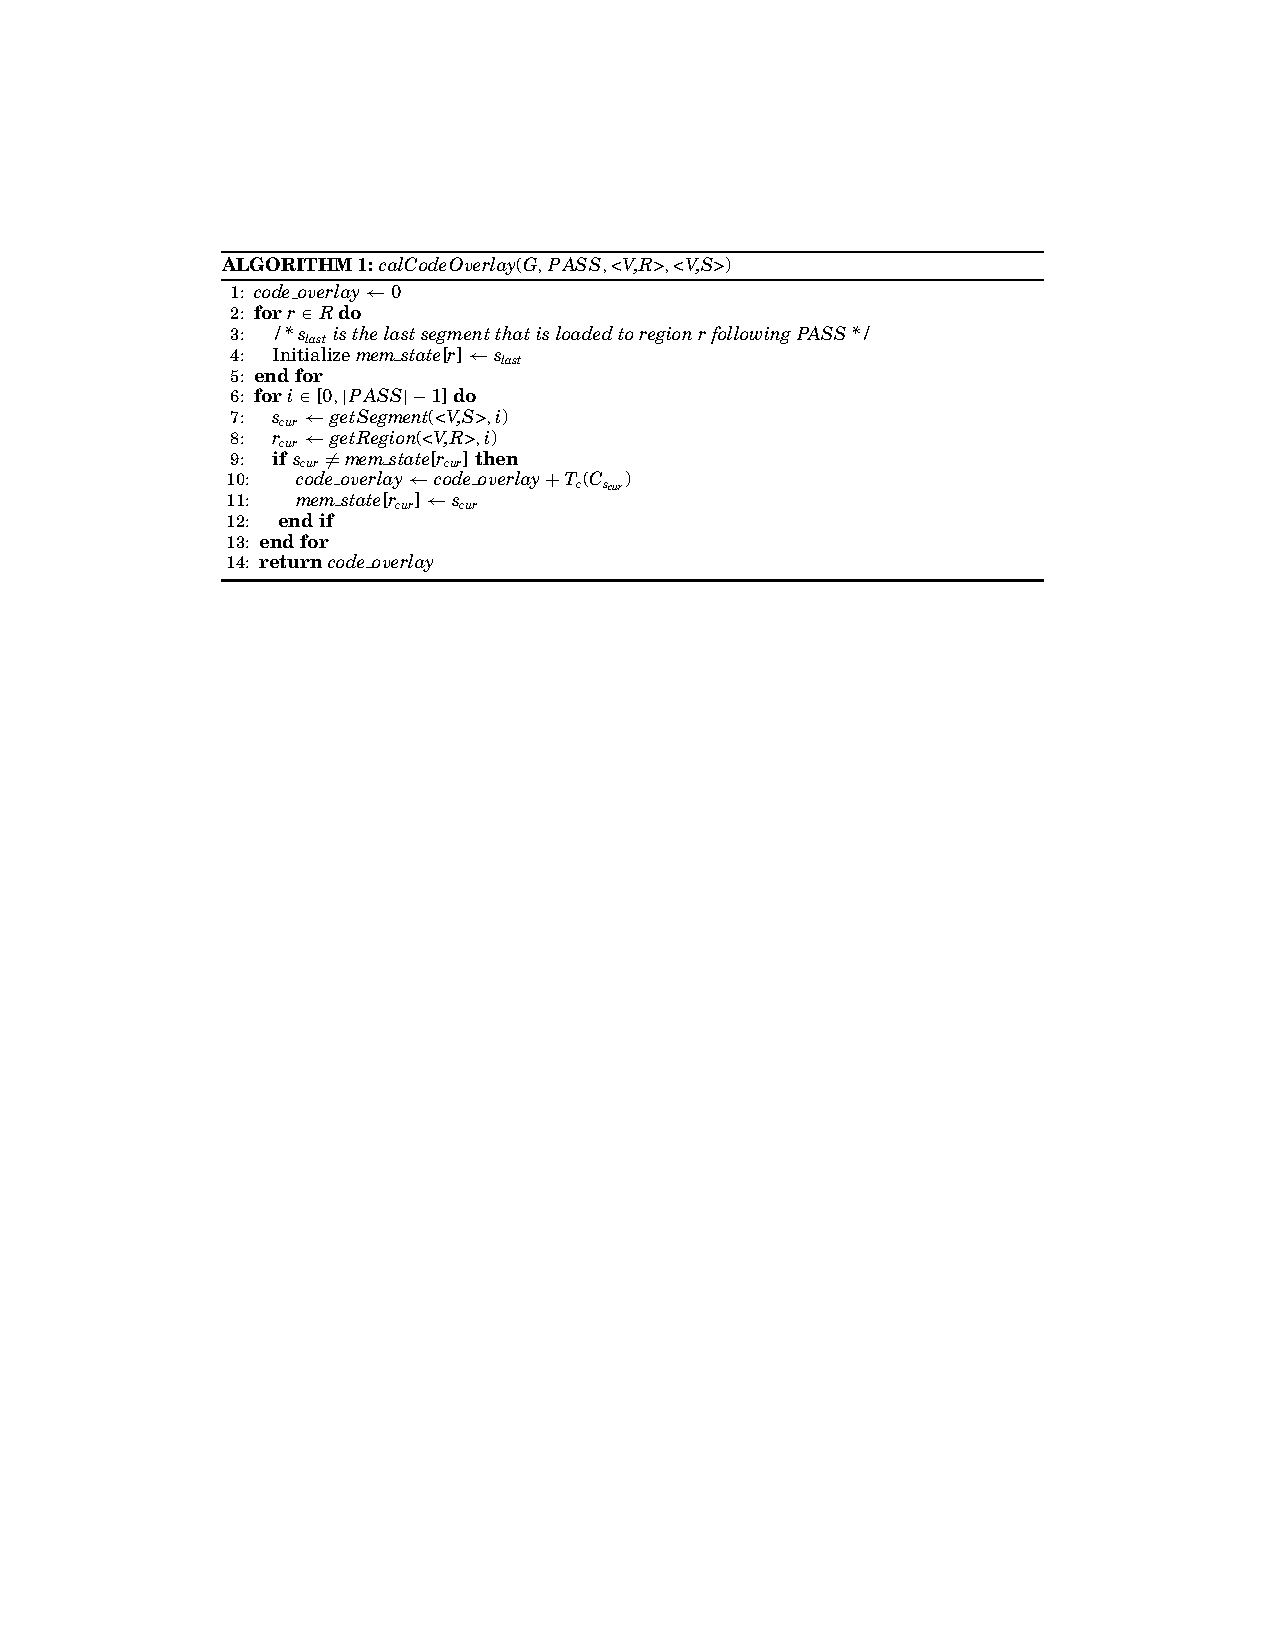
\includegraphics[width=1.2\textwidth]{algo1} % TODO extract algo
  \end{center}
\end{frame}

\end{document}
